\documentclass{tufte-handout}
\usepackage{amsmath,amsthm}


\usepackage{pgfplots}
\pgfplotsset{width=\textwidth,compat=1.5.1}

\newtheorem{claim}{Claim}[section]
\title{\sf Approximation Algorithm for Maximum Cut}
\date{}

\begin{document}
\maketitle

\section{Maximum Cut}
Consider an undirected graph $G=(V,E)$ with positive edge weights
$w(e)$ $(e\in E)$.
Set $n=|V|$ and $m=|E|$.
The Maximum Cut problem (Maxcut) is to find a partition of the
vertices with the largest total weight of the edges ``crossing'' the
partition, i.e., maximising the value of \[c(A)= \sum_{(u,v)\in E,
  u\in A, v\notin A} w(u,v)\,\] over all $A\subseteq V$.

Maxcut is NP-hard, so we have little hope of writing an algorithm that
solves arbitrary Maxcut instances optimally.

\subsection{ Algorithm R}

Consider the following simple randomized algorithm (call it
Algorithm~R): Let $A$ be a \emph{random subset} of $V$ constructed by
flipping a coin $r(v)\in\{0,1\}$ for every vertex $v\in V$ and setting
$v\in A$ if and only if $r(v)=1$.

\subsection{Inputs}
The  data directory contains two input instances:
\begin{description}
\item[ pw09\_100.9.txt:] A random instance with $|V|=100$ and
  $|E|=4455$. The best cut in this instance is
  13658.\sidenote{A. Wiegele, Biq Mac Library - A collection of Max-Cut
    and quadratic 0-1 programming instances of medium size, 2007.}
\item[ matching\_1000.txt:] A disjoint union of 500 edges with unit weight.
\end{description}

The input format is straightforward: the first line contains $n$ and
$m$; every following line describes an edge in the format first
vertex, second vertex, weight.
All weights are integers, vertices are numbered $1,2,\ldots, n$.

\subsection{Algorithm S}
Consider the following simple greedy swapping algorithm (call it 
Algorithm~S): Let all the verticies be outside of $A$ to begin with.
A vetrex can be swapped, which means that if it's outside of $A$ its moved into
$A$ and if its inside $A$ its moved out of $A$.
Pick the first vertex you can find that increases your cut if swapped.
Swap this vetrex, and continue doing so until no vertex increases the cut
if swapped, eg you find a local maxima.

\subsection{Algorithm RS}
Consider the following simple randomized swapping algorithm (call
it Algorithm~RS): Combine Algorithm R and S by instead of placing
all vertices outside of $A$ to begin with in S, place the verticies according
to the output of R. Then proceed with the swapping part of S.

\subsection{ Deliverables}

\begin{enumerate}
\item Implement algorithm R, S and RS and run it on the dataset provided in
  the data directory.
  Use whatever programming language and libraries you want, but make
  sure that your code is short and crisp; Each of the algorithms should 
  not be much more than 20 lines. Reading input + scoring should also be
  small. Making all the code together less than 100 lines is a suitable goal.
  Attach a printout of the code to the report.
\item Fill out the report on the next page; you can just use the
  \LaTeX\ code if you want.
\end{enumerate}

\newpage


\newpage
\section{Maxcut Lab Report}


by Alice Cooper and Bob Marley\sidenote{Complete the report by filling
  in your names and the parts marked $[\ldots]$.
  Remove the sidenotes in your final hand-in.}

\subsection{Running time}

\begin{tabular}{ c c c }
    Algorithm~R & Algorithm~S & Algorithm~RS \\ 
    $[\ldots]$ & $[\ldots]$ & $[\ldots]$ 
\end{tabular}\sidenote{Replace each
  $[\ldots]$ by a function of a subset of the parameters $\{n, m, W\}$, where $W = \sum_{e \in E}w(e)$.
  Use asymptotic notation.}

\subsection{Randomness}

Algorithm R uses $[\ldots]$\sidenote{Replace
  $[\ldots]$ by a function of $n$ and/or $m$. Do not use asymptotic
  notation. This is supposed to be easy.} random bits.

\subsection{Solution quality}

\paragraph{Experiments.}

\begin{enumerate}
\item
For the input file  pw09\_100.9.txt with $t=100$ runs, we found
for each algorithm, the average cutsize $Avg(C)$ and the maximum cutsize $Max(C)$:

\begin{tabular}{ l c c }
    Algorithm & $Avg(C)$ & $Max(C)$ \\ 
    R & $[\ldots]$ & $[\ldots]$ \\
    S & $[\ldots]$ & $[\ldots]$ \\
    RS & $[\ldots]$ & $[\ldots]$
\end{tabular}\sidenote{Replace each $[\ldots]$
with the values obtained by running your experiments.}
\medskip

The optimum was given to us as $\operatorname{OPT} = 13658$.

\medskip

The distribution of cutsizes for Algorithm~R looks as follows:\sidenote{Display your
  cutsizes as a histogram. Use whatever software you like to produce
  the image; the placeholder image on the left is constructed in the
  \LaTeX\ source.}

\medskip

\noindent
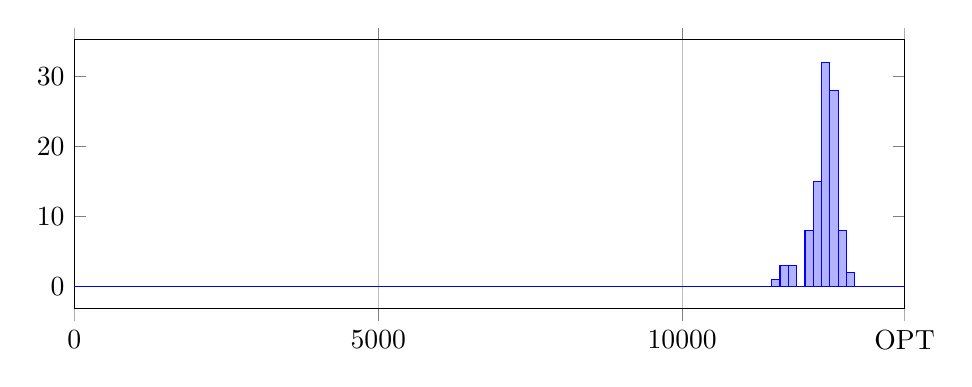
\begin{tikzpicture}
\begin{axis}[
  height= 5cm,
  ybar interval,
  xmin = 0,  xmax = 13658,
  xtick =       {0   ,   5000,   10000, 13658},
  xticklabels = { $0$, $5000$, $10000$,   OPT},
  x tick label as interval = false,
  scaled ticks = false
]
    \addplot+[hist={bins=100}]
        table[y index=0] {
          % output of 
          % perl -e "for $i (1..100) { system 'python sol/rmaxcut.py < data/pw09_100.9.txt '}"
12296
12401
12176
12414
11767
12458
12407
12551
12363
12526
11865
12353
12159
12504
12130
11616
12347
12201
12473
12368
12196
12274
12064
12398
12733
12620
12402
12231
12442
12360
12567
11650
12334
12543
12108
12523
12256
12524
12642
12040
12404
12408
12606
12094
12484
12457
12459
12326
12307
12282
12276
12459
12107
12474
12410
12109
12308
12471
12588
12473
12338
12499
12233
12453
12448
12541
12488
12497
12230
12393
12335
12446
11503
12304
12612
12378
12108
12684
12422
12557
12441
12334
12400
12369
11734
12237
12631
12289
11773
12460
12366
12355
12502
12323
12543
12271
12415
12227
12711
12370
    };
\end{axis}
\end{tikzpicture}

The distribution of cutsizes for Algorithm~RS looks as follows: $[\ldots]$
\sidenote{Display a plot similar to the histogram for Algorithm~R, but instead for Algorithm~RS.}

\item
For the input file matching\_1000.txt
$[\ldots]$\sidenote{Perform the same analysis for 
    matching\_1000.txt. This involves thinking to determine OPT.}
\end{enumerate}


\paragraph{Analysis of performance guarantee}

Clearly, Algorithm~R performs quite badly on input 
  matching\_1000.txt.
We will show that it can perform \emph{no worse} than that, i.e., we
will establish that in expectation, the cutsize $C$ satisfies $C \geq
[\ldots]\cdot \operatorname{OPT}$.\sidenote{Replace [\ldots] by the
  right constant}


We will view $C$ as a random variable that gives the size of the cut
defined by the random choices.
Let $W$ denote the total weight of the edges of $G$, i.e.,
\[ W= \sum_{e\in E} w(e)\,.\]

Then,
\begin{equation}\label{eq: E[C]}
E[C] = \textstyle\frac{1}{2}\cdot W\,.
\end{equation}

To see this, define the indicator random variable $X_{uv}$ for every
edge $uv\in E$ as follows.
Set $X_{uv}=1$ if $uv$ crosses the cut, i.e., $u\in A$ and $v\notin A$
or $u\notin A$ and $v\in A$.
Otherwise, $X_{uv} = 0$.

Then, $\Pr(X_{uv} = 1) = [\ldots]$.
Now, $E[C]=[\ldots]$ Finally, we have 
\(E[C]\geq [\ldots]\cdot \text{OPT}\) because clearly
$[\ldots]$.\sidenote{Fill in the missing blanks in this paragraph.
  Your calculations and arguments need to include phrases like
  ``because BLA and BLA are independent'' or ``disjoint,'' and ``by
  linearity of expectation'' and ``because the weights are positive.''
}

\bigskip
Algorithms~S and RS perform very well on input matching\_1000.txt. In fact
both algorithms always find the optimum. The reason for this is that $[\ldots]$
\sidenote{Explain why the optimum is always found.}.

However Algorithm~RS does not always find the optimum even for all bipartite graphs. 
An example of this scenario is the graph $G$,
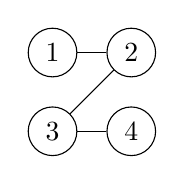
\begin{tikzpicture}[every node/.style={draw,circle}]
  \node (1) at (0,1)  { 1 };
  \node (2) at (1,1)  { 2 };
  \node (3) at (0,0) { 3 };
  \node (4) at (1,0) { 4 };
  \draw[-] (1) edge (2);
  \draw[-] (2) edge (3);
  \draw[-] (3) edge (4);
\end{tikzpicture}

\bigskip

Where the weight of the edges are

\medskip

\begin{tabular} {c c c}
    u & v & weight \\
    1 & 2 & $[\ldots]$ \\
    2 & 3 & $[\ldots]$ \\
    3 & 4 & $[\ldots]$
\end{tabular}\sidenote{Fill in weights of the edges in the graph such 
that the graph has a local maxima less than the global maxima.}
\medskip

Here if nodes $[\ldots]$ are inside $A$, Algorithm~RS gets stuck in a local maxima of size $[\ldots]$. The global maxima has size $[\ldots]$, with nodes $1$ and $3$ inside $A$.\sidenote{Fill in the blanks so the sentence makes sense.}

\newpage
\section{Perspective}
To establish that Maxcut is NP-hard one reduces from NAE-Sat, a
reduction that can be found in many places\sidenote{C. Moore and
S. Mertens, \emph{The Nature of Computation}, Oxford University Press,
  2011, p. 146.}
Recall that the related problem \emph{Minimum Cut} is easy because of
the max flow--min cut theorem.
A moment's thought should convince you that as soon as negative
weights are allowed, the two problems are the same (and both are
hard).
Algorithm R doesn't work at all for negative weights.

Algorithm R is a classical randomised approximation algorithm, its
origins seem to be shrouded in the mists of time.
The \emph{deterministic} algorithm of Sahni and Gonzales\sidenote{S.\
  Sahni and T.\ Gonzalez.
  P-complete approximation problems.
  \emph{J.\ Assoc.\ Comput.\ Mach.}, 23(3):555--565, 1976.}
can be viewed as a derandomisation of R using the \emph{method of
  conditional expectations}.
These algorithms were best knows until the breakthrough result of
Goemans and Williamson,\sidenote{M.\ X.\ Goemans and D.\ P.\
  Williamson.
  Improved approximation algorithms for maximum cut and satisfiability
  problems using semidefinite programming.
  \emph{J.\ Assoc.\ Comput.\ Mach.}, 42(6):1115--1145, 1995.}
which improved the approximation factor to $0.87856$.
H\aa{}stad has shown that no algorithm can approximate the maxcut
better than $16/17\sim 0.941176$ unless P equals NP. Khot has shown
that the Goemans--Williamson bound is essentially optimal under the
\emph{Unique Games Conjecture}.

\end{document}